%==============================================================================
\chapter{Methodik}
\label{chap:methodik}
%==============================================================================
Ziel dieser Arbeit ist die Entwicklung einer Methode für die Modellierung von Kraftstoffsystemen für Fluggasturbinen, um deren Vorauslegung zu unterstützen. Insbesondere wird angestrebt, eine Vergleichbarkeit des Wärme-/Leistungsbedarfs zwischen Wasserstoff- und Kerosin-Kraftstoffsystemen zu ermöglichen. 

Zunächst werden die Stoffmodelle für Kerosin und Wasserstoff erläutert. Anschließend werden die für die Modellierung der Kraftstoffsysteme erforderlichen Komponentenmodelle definiert. Im nächsten Schritt wird das Kraftstoffsystem des kerosinbetriebenen CFM56-5B Triebwerks aus den Komponentenmodellen nachgebildet und mögliche Architekturen für Wasserstoff-Kraftstoffsysteme erarbeitet.

\section{Annahmen und Vereinfachungen}

Um einen Kompromiss zwischen Detailtiefe, Genauigkeit und Rechenaufwand zu finden, werden in dieser Arbeit mehrere Vereinfachungen verwendet. Insbesondere gelten die betrachteten Modelle lediglich für den stationären Fall. Transientes Systemverhalten wird nicht betrachtet. 

Zudem wird in den für die Modellierung relevanten Querschnitten der Kraftstoffsysteme von vernachlässigbaren Geschwindigkeiten, beziehungsweise kinetischen Energien ausgegangen. Innerhalb der modellierten Turbomaschinen ist diese Annahme nicht gültig, jedoch beschränkt sich die Modellierung auf die Erfassung der Stoffgrößen in den Leitungen zwischen den jeweiligen Komponenten. Bei einer konservativ abgeschätzten Machzahl in den Leitungen von $Ma_L=0.1$ und mit dem Isentropenexponenten $\kappa_{\mathrm{H}_2} = 1.4$ beträgt das mit der Isentropenbeziehung berechnete total zu statische Temperaturverhältnis  $\frac{T_{t,L}}{T_L}$

\begin{equation}\label{Eq:mach}
	\frac{T_{t,\mathrm{L}}}{T_\mathrm{L}}=1+\frac{\kappa_{\mathrm{H}_2}-1}{2}Ma_\mathrm{L}^2
\end{equation}

lediglich $1,002$. Unter Annahme eines maximalen Wasserstoffmassenstroms von \SI{0.731}{\kg\per\s} bei einer Temperatur von \SI{300}{\K} beträgt der maximale Leitungsdurchmesser \SI{69}{\milli\m}, was als unkritisch eingestuft wird. Somit gilt die Annahme 

\begin{equation}\label{Eq:ts}
	T_s=T_t=T,\quad h_s=h_t=h,\quad p_s=p_t=p\,.
\end{equation}

\section{Stoffmodelle}

Die Modellierung der Kraftstoffsysteme erfordert Stoffmodelle, um thermodynamische Zustandsgrößen wie die spezifische Enthalpie und Entropie in Abhängigkeit von Temperatur und Druck der Kraftstoffe zu bestimmen. In diesem Abschnitt werden die für Kerosin und Wasserstoff verwendeten Stoffmodelle erläutert.

\subsection{Wasserstoff Stoffmodell}

Wasserstoff besteht aus zwei unterschiedlichen Kernspin-Isomeren, Parawasserstoff und Orthowasserstoff. Da sich die beiden Spin-Isomer in ihrer Wärmekapazität bei niedrigen Temperaturen unterscheiden, muss das Stoffmodell das Verhältnis der Kern-Isomer berücksichtigen. Bei Temperaturen oberhalb von \SI{200}{\K} liegen die Isomere im thermischen Gleichgewicht in einem Verhältnis von 3:1 zwischen Ortho- und Parawasserstoff vor. Flüssiger Wasserstoff besteht im Gleichgewichtszustand hingegen aus nahezu purem Parawasserstoff (Siehe Abbildung \ref{fig:spin}). In Abwesenheit eines Katalysators wird der Gleichgewichtszustand nur langsam erreicht. Es ist daher davon auszugehen, dass der ursprünglich kryogen gelagerte Wasserstoff im gesamten Kraftstoffsystem nahezu vollständig in Form von Parawasserstoff vorliegt. Für die Parametrierung des Stoffmodells wird daher eine Zusammensetzung aus purem Parawasserstoff angenommen. \cite{Buntkowsky.2022}

\begin{figure}[ht]
	\centering
	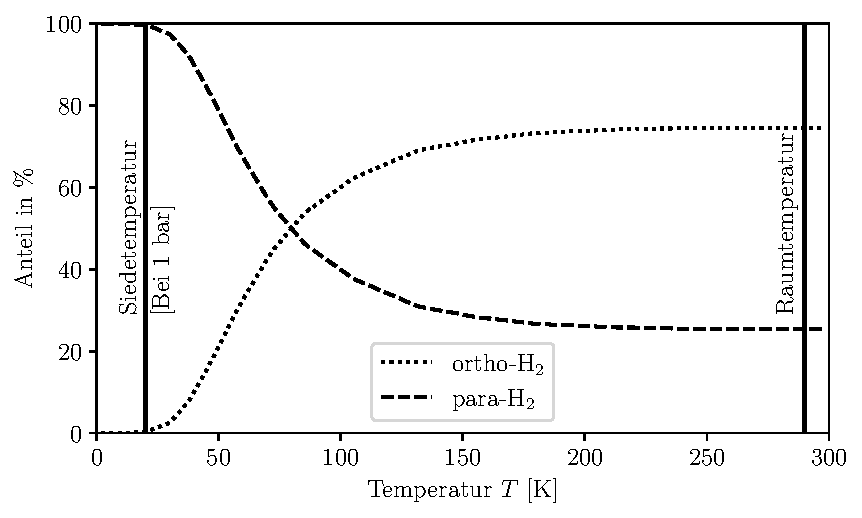
\includegraphics[width=1\linewidth]{4_Abbildungen/2_Hauptteil/spin.pdf}
	\caption{Wasserstoff Kernspin-Isomer Anteile nach \cite{Buntkowsky.2022}}
	\label{fig:spin}
\end{figure}
\FloatBarrier 

Für die Berechnung der thermodynamischen Zustandsgrößen von Parawasserstoff, wird ein am Institut für Strahlantriebe und Turbomaschinen (IST) entwickeltes Stoffmodell weiterentwickelt. Das Stoffmodell basiert auf einem von Leachman et al. \cite{Leachman.2017} beschriebenen Ansatz, der die Zustandsgrößen in Abhängigkeit der Helmholtz-Energie, die auch als freie Energie bekannt ist, setzt. Leachman et al. berechnen die entdimensionierte Helmholtz-Energie $\alpha$ 

\begin{equation}\label{Eq:free-energy}
	\alpha(\delta, \tau) = \alpha^0(\delta, \tau) + \alpha^r(\delta, \tau)
\end{equation}

als Summe der Idealgaskomponente $\alpha^0$ und des Anteils aufgrund von Kompressibilität $\alpha^r$. Hierbei gelten folgende Definitionen der entdimensionierten Helmholtz-Energie $\alpha$ und der entdimensionierten Variablen $\delta$ und $\tau$

\begin{equation}
	\alpha = \frac{a}{RT}, \quad \delta = \frac{\rho}{\rho_c}, \quad \tau = \frac{T_c}{T} \,
\end{equation}

in Abhängigkeit der spezifischen freien Energie $a$ und den Zustandsgrößen $\rho_c, T_c$ im kritischen Punkt.  Leachman et al. berechnen die Idealgaskomponente der entdimensionierten freien Energie $\alpha^0$

\begin{equation}\label{Eq:free-energy-idealgas}
	\alpha^0(\tau,\delta)=ln(\delta)+(a_0-1)\mathrm{ln}(\tau)+a_1+a_2\tau-\sum_{i=3}^{m}a_i\frac{(\frac{T_c}{\tau})^{k_i}}{k_i(k_i+1)}+\sum_{i=m+1}^{n}a_i\mathrm{ln}\left(1-e^{\frac{-k_i\tau}{T_c}}\right) \,
\end{equation}

mit einer semi-empirischen Zustandsgleichung, wobei die empirisch bestimmten Koeffizienten $a_i$ und $k_i$ verwendet werden. Die Zustandsgleichung für den Anteil an der entdimensionierten freien Energie aufgrund von Kompressibilitätseffekten $\alpha^r$

\begin{equation}\label{Eq:free-energy-compressibility}
	\alpha^r(\tau,\delta)=\sum_{i=1}^{l}N_i\delta^{d_i}\tau^{t_i}+\sum_{i=l+1}^{m}N_i\delta^{d_i}\tau^{t_i}e^{-\delta^{p_i}}+\sum_{i=m+1}^{n}N_i\delta^{d_i}\tau^{t_i}e^{-\phi_i(\delta-D_i)^2-\beta_i(\tau-\gamma_i)^2)}
\end{equation}

orientiert sich an theoretischen und praktischen Abwägungen. Die in Gleichung \ref{Eq:free-energy-compressibility} enthaltenen Koeffizienten $N_i, d_i, t_i, p_i, \phi_i, D_i, \beta_i$ und $\gamma_i$ werden experimentell bestimmt. Da die freie Energie eine Funktion von Dichte und Temperatur ist, der Zustand in dieser Arbeit hingegen in Form von Druck und Temperatur bekannt ist, wird zunächst die Dichte des Wasserstoffs berechnet. Um die Dichte zu berechnen wird die Zustandsfunktion für den Druck $p$

\begin{equation}\label{Eq:pressure-guess}
	p=\rho RT\left(1+\delta\frac{\partial\alpha^r}{\partial\delta}(\delta, \tau)\right)
\end{equation}

iterativ mit dem Newton-Raphson-Verfahren gelöst. Die Ableitung des inkompressiblen Anteils der freien Energie nach der entdimensionierten Dichte $\frac{\partial\alpha^r}{\partial\delta}$ wird aus Gleichung \ref{Eq:free-energy-compressibility} hergeleitet. Mit Dichte und Temperatur beziehungsweise deren entdimensionierten Äquivalenten ist es möglich die freien Energien und die Ableitungen der freien Energien nach $\delta$ und $\tau$ zu berechnen und das Stoffmodell ist somit eindeutig bestimmt. Diese Werte liefern die Grundlage für die Berechnung der thermodynamischen Zustandsgrößen mit den in Tabelle \ref{Tab:thermodynamic_properties_h2} definierten Zustandsgleichungen.

\begin{table}[ht]
	\centering
	\caption{Formeln für thermodynamische Zustandsgrößen von Wasserstoff}
	\begin{tabular} {|l|c|c|} \hline%
		\multicolumn{2}{|c|}{Zustandsgröße}  & Formel\\ \hline\hline%
		spezifische Enthalpie &$h$ 		  & $RT(\tau\frac{\partial\alpha}{\partial\tau}+\delta\frac{\partial\alpha^r}{\partial\delta}+1)$ \\ \hline%
		spezifische Entropie& $s$ 		      &  $R(\tau\frac{\partial\alpha}{\partial\tau}-\alpha)$\\ \hline%
		spezifische isochore Wärmekapazität &$c_v$ 	    &  $-R\tau^2\frac{\partial^2\alpha}{\partial\tau^2}$\\ \hline%		
		spezifische isobare Wärmekapazität &$c_p$        &  $c_v+R\frac{\left(1+\delta\frac{\partial\alpha^r}{\partial\delta}-\delta\tau\frac{\partial^2\alpha^r}{\partial\delta\partial\tau}\right)^2}{1+2\delta\frac{\partial\alpha^r}{\partial\delta}+\delta^2\frac{\partial^2\alpha^r}{\partial\delta^2}}$\\ \hline%
	\end{tabular}	
	\label{Tab:thermodynamic_properties_h2}%
\end{table}
\FloatBarrier 

\subsection{Kerosin Stoffmodell}

Die Modellierung von Kerosin beziehungsweise Jet-A ist grundsätzlich mit Unsicherheit behaftet, da die Spezifikation des Kraftstoffs vergleichsweise große Abweichungen der Eigenschaften zulässt. Outcalt et al. \cite{Outcalt.2009} haben die Dichte von drei unterschiedlichen Proben an Jet-A Kraftstoff für Temperaturen zwischen \SI{270}{\K} und \SI{470}{\K} und Drücke zwischen \SI{83}{\kilo\Pa} und \SI{30}{\mega\Pa} gemessen und haben Abweichungen von bis zu $4\,\%$ zwischen den Dichten der Proben ermittelt.

Da Kerosin kein Reinstoff, sondern eine Mischung von Kohlen-Wasserstoffverbindungen mit unterschiedlichen Kettenlängen ist, kann ein Kerosin Stoffmodell nicht mit demselben Ansatz wie das Wasserstoff Stoffmodell entwickelt werden. Stattdessen wird ein empirisches Stoffmodell verwendet, das von McBridge et al. \cite{McBridge.2002} vorgeschlagen wurde. Die Autoren haben generische empirische Formeln in Form von Polynomen für die Enthalpie, Entropie und isobare Wärmekapazität aufgestellt und anhand experimenteller Messungen der Zustandsgrößen für 2000 Spezies, inklusive Jet-A Kraftstoff, mit den Koeffizienten $a_i$ und $b_i$ parametriert. Tabelle \ref{Tab:thermodynamic_properties_jeta} liefert einen Überblick über die verwendeten Zustandsgleichungen.

\begin{table}[ht]
	\centering
	\caption{Thermodynamische Zustandsgrößen von Jet-A Kraftstoff nach 
		\cite{McBridge.2002}}
	\begin{tabular} {|l|c|l|} \hline%
		\multicolumn{2}{|c|}{Zustandsgröße}  & Formel\\ \hline\hline%
		spezifische Enthalpie &$h$ & $R(a_1T^{-2}+a_2T^{-1} +a_3$ \\ 
		& & $+a_4T+a_5T^2+a_6T^3+a_7T^4)$\\ \hline
		spezifische Entropie& $s$ &  $R(-a_1T^{-1}+a_2ln(T)+a_3T$\\ 
		& & $+\frac{a_4T^2}{2}+\frac{a_5T^3}{3}+\frac{a_6T^4}{4}+\frac{a_7T^5}{5}+b_1)$\\ \hline
		spezifische isobare Wärmekapazität &$c_p$ &  $R(-\frac{a_1T^{-2}}{2}-a_2T^{-1}+a_3ln(T)+ a_4T$\\ 
		& & $+\frac{a_5T^{2}}{2}+\frac{a_6T^{3}}{3}+\frac{a_7T^{4}}{4}+b_2)$\\ \hline
	\end{tabular}	
	\label{Tab:thermodynamic_properties_jeta}%
\end{table}
\FloatBarrier 

Da eine Berechnung der Dichte mit demselben Ansatz nicht möglich ist, werden in dieser Arbeit stattdessen von Outcalt et al. \cite{Outcalt.2009} gemessenen Datenpunkte interpoliert. Als Datengrundlage wird die Probe "Jet-A 4658" verwendet, da sie von den Autoren als die repräsentativste der Proben erachtet wird. Für die Interpolation werden die vier angrenzenden Datenpunkte herangezogen. Zunächst wird die Dichte für den Druck interpoliert, da die Autoren die Dichte für uneinheitliche Druckschritte gemessen haben. Abschließend werden die druck-interpolierten Punkte für die Temperatur interpoliert. 

% Für die Berechnung der Dichte $\rho(T,p)$, werden die vier angrenzenden gemessenen Dichten $\rho(T_\mathrm{N},p_{\mathrm{N,n}})$, $\rho(T_\mathrm{N},p_{\mathrm{N,h}})$, $\rho(T_\mathrm{H},p_{\mathrm{H,n}})$ und $\rho(T_\mathrm{H},p_{\mathrm{H,h}})$ benötigt. Bei der Extrapolation werden stattdessen Messwerte der jeweils zwei nächsthöheren Temperaturen als Stützstellen verwendet. Da Outcalt et al. die Dichte für einheitliche Temperaturschritte, aber uneinheitliche Druckschritte gemessen haben, werden zunächst die Dichten $\rho(T_\mathrm{H}, p)$ und $\rho(T_\mathrm{N}, p)$ 

% \begin{equation}\label{Eq:pressure-interp}
	%\rho(T_i, p)= \rho(T_i, p_{i,\mathrm{n}}) + \frac{\rho(T_i, p_{i,\mathrm{h}})-\rho(T_i, p_{i,\mathrm{n}})}{p_{i,\mathrm{h}}-p_{i,\mathrm{n}}}(p-p_{i,\mathrm{n}}) 
%\end{equation}

%für den Druck interpoliert. Abschließend wird die Dichte $\rho(T,p)$

%\begin{equation}\label{Eq:temperature-interp}
	%\rho(T, p)= \rho(T_\mathrm{N}, p) + \frac{\rho(T_\mathrm{H}, p)-\rho(T_\mathrm{N}, p)}{T_\mathrm{H}-T_\mathrm{N}}(T-T_\mathrm{N}) 
%\end{equation}

%für die Temperatur interpoliert. 


\section{Modellierung der Komponenten}

Im Folgenden werden die Modellierungen der verschiedenen Kraftstoffsystem-Komponenten erläutert. Neben Modellen für Verdichter und Pumpen wird ein Modell für Wärmeübertrager benötigt. Für die Modellierung der Wasserstoff-Kraftstoffsysteme ist zusätzlich ein Modell für parallele Wasserstoffverbrennung in einer Nebenbrennkammer erforderlich. 

\subsection{Pumpen und Verdichter}

Sämtliche Verdichter- und Pumpentypen werden durch die Definition des isentropen Wirkungsgrad $\eta_s$

\begin{equation}\label{Eq:isentropic}
	\eta_s=\frac{h_2-h_1}{h_{2,s}-h_1}
\end{equation}

modelliert. Dabei werden neben dem isentropen Wirkungsgrad auch der Austrittsdruck $p_2$, der Eintrittsdruck $p_1$, die Eintrittstemperatur $T_1$ und somit über das Stoffmodell die spezifische Eintrittsenthalpie $h_1(T_1, p_1)$ sowie die spezifische Eintrittsentropie $s_1(T_1, p_1)$ als bekannt vorausgesetzt. Die Austrittstemperatur des reversiblen Prozesses $T_{2,s}$ wird iterativ mit der spezifischen Eintrittsentropie $s_1$ und dem Austrittsdruck $p_2$ bestimmt. Die Temperatur der nächsten Iteration wird mit der idealen Zustandsgleichung für die Entropie und der spezifischen isobaren Wärmekapazität $c_p(T_1,p)$ geschätzt 

\begin{equation}\label{Eq:entropy}
	s(T_2,p)-s(T_1, p)=\cancel{s(T_0,p_0) - s(T_0,p_0)} + c_p(T_1,p) ln\left(\frac{T_2}{T_1}\right) - {\cancel{\overbrace{R ln\frac{p}{p}}^{\substack{\text{Nur bei } \\ \text{idealem Gas}}}}}\,.
\end{equation}


Aus der Austrittstemperatur $T_{2,s}$ folgt direkt die spezifische Austrittsenthalpie $h_{2,s}$ des reversiblen Prozesses und somit durch Gleichung \ref{Eq:isentropic} auch die spezifische Austrittsenthalpie $h_2$ des realen Prozesses. In einem weiteren Iterativen Prozess wird mit dem Austrittsdruck $p_2$ und der spezifischen Austrittsenthalpie $h_2$ die Austrittstemperatur $T_2$ berechnet. Auch hier wird das ideale Stoffmodell verwendet, um Werte für die Austrittstemperatur zu schätzen

\begin{equation}\label{Eq:enthalpy}
	h(T_2,p)-h(T_1,p)=\cancel{h(T_0,p_0) - h(T_0,p_0)} + c_p(T_1,p)(T_2 - T_1) - {\cancel{\overbrace{v(p-p)}^{\substack{\text{Nur bei idealer} \\ \text{Flüssigkeit}}}}}\,.
\end{equation}

Abschließend wird mit der Energiebilanz um die Pumpe beziehungsweise den Verdichter die Leistung $P$ 

\begin{equation}\label{Eq:power}
	P=\dot{m}(h_2-h_1)
\end{equation}

bestimmt, die benötigt wird, um den Kraftstoffmassenstrom $\dot{m}$ zu fördern.

\subsection{Wärmeübertrager}

Eine Auslegungsrechnung der Wärmeübertrager wird in dieser Arbeit nicht angestrebt. Es gilt jedoch die Randbedingung, dass die Wärmequelle eines Wärmeübertragers in jedem Schnitt ein höheres Temperaturniveau als der zu erwärmende Kraftstoffmassenstrom aufweist. Anhand des $\dot{Q}-T$ Diagramms (Beispiel siehe Abbildung \ref{fig:hx}) kann festgestellt werden, ob über den gesamten Wärmeübertrager eine minimale Temperaturdifferenz $\Delta T_{min}$ zwischen Wärmequelle und Kraftstoffstrom eingehalten werden kann.


\begin{figure}[ht]
	\centering
	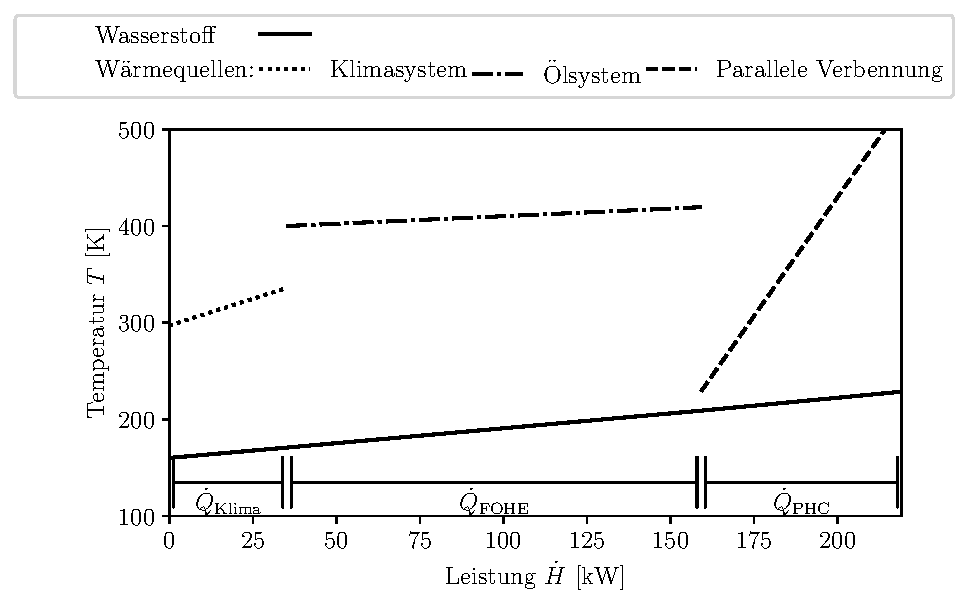
\includegraphics[width=1\linewidth]{4_Abbildungen/2_Hauptteil/hx.pdf}
	\caption{schematisches Wärmestromdiagramm eines Kraftstoffsystems}
	\label{fig:hx}
\end{figure}
\FloatBarrier 

Aus dem Eintrittszustand des Kraftstoffs in den Wärmeübertrager $T_1, p_1$ ergibt sich die spezifische Enthalpie des Kraftstoff im Eintritt in den Wärmeübertrager $h_1$. Die spezifische Austrittsenthalpie $h_2$

\begin{equation}\label{Eq:energy-hx}
	h_2=h_1 +q=h_1+\frac{\dot{Q}}{\dot{m}}
\end{equation}

erschließt sich direkt aus der Energiebilanz der Kraftstoffseite des Wärmeübertragers mit dem Wärmestrom $\dot{Q}$ und dem Kraftstoffmassenstrom $\dot{m}$. Über den Wärmeübertrager besteht infolge von Strömungsverlusten ein Druckverhältnis $\pi$. Der Austrittsdruck $p_2$

\begin{equation}\label{Eq:pressuredrop}
	p_2 = p_1 \pi
\end{equation}

fällt somit geringer als der Eintrittsdruck aus. Im Rahmen dieser Arbeit wird für das Druckverhältnis $\pi$ ein konstanter Wert angenommen. Abschließend wird erneut Gleichung \ref{Eq:enthalpy} eingesetzt, um iterativ die Austrittstemperatur $T_2$ des Kraftstoffs aus dem Wärmeübertrager zu bestimmen.

\subsection{Kraftstoffmischung}

In der Kraftstoffmischung werden die Kraftstoffmassenströme $\dot{m}_{1,\mathrm{\rom{1}}}$ und $\dot{m}_{1,\mathrm{\rom{2}}}$, mit demselben Eintrittsdruck $p_1$, aber unterschiedlichen Eintrittsenthalpien $h_{1,\mathrm{\rom{1}}}, h_{1,\mathrm{\rom{2}}}$ miteinander vermischt. Der Austrittsmassenstrom $\dot{m}_2$

\begin{equation}\label{Eq:mass}
	\dot{m}_2 = \dot{m}_{1,\mathrm{\rom{1}}}+\dot{m}_{1,\mathrm{\rom{2}}}
\end{equation}

berechnet sich aus der Massenbilanz um die Mischung. Die Austrittsenthalpie der Kraftstoffmischung 

\begin{equation}\label{Eq:energy-mix}
	h_{2} = \frac{\dot{m}_{1,\mathrm{\rom{1}}}h_{1,\mathrm{\rom{1}}}+\dot{m}_{1,\mathrm{\rom{2}}}h_{1,\mathrm{\rom{2}}}}{\dot{m}_2}
\end{equation}

wird mit der Energiebilanz um die Mischung bestimmt. Druckverluste in der Mischung werden vernachlässigt, somit entspricht der Austrittsdruck $p_2$, dem Eintrittsdruck $p_1$. Abschließend wird Gleichung \ref{Eq:enthalpy} erneut eingesetzt, um iterativ die Austrittstemperatur $T_2$ des gemischten Kraftstoffmassenstroms zu bestimmen. 

\subsection{Parallele Wasserstoffverbrennung}

In den Wasserstoff-Kraftstoffsystemen ist nicht ausreichend Abwärme vorhanden, um den Wasserstoff auf beliebige Brennkammer-Eintrittstemperatur zu erwärmen. In dieser Arbeit wird der potenzielle zusätzliche Wärmebedarf durch parallele Wasserstoffverbrennung in einer separaten Brennkammer aufgebracht. Diese Brennkammer wird mit Wasserstoff von der Kraftstoffregeleinheit und mit Fan-Zapfluft versorgt. Die Modellierung der parallelen Wasserstoffverbrennung berechnet diesen Mehrbedarf an Wasserstoff und Zapfluft. Unter Abwägung der angestrebten Detailtiefe werden die Prozesse der parallelen Wasserstoffverbrennung mit einer vereinfachten Energiebilanz um die Nebenbrennkammer und den dazugehörigen Wärmeübertrager modelliert 

\begin{equation}\label{Eq:phc}
	0 = \dot{m}_{\mathrm{H}_2, \mathrm{PHC}}\left(H_{u, \mathrm{H}_2} + \frac{1}{\beta_\mathrm{PHC}}c_{p,\mathrm{L}} T_\mathrm{Z} - \left(1+\frac{1}{\beta_\mathrm{PHC}}\right)c_{p,\mathrm{B}} T_\mathrm{W}\right)-\dot{Q}_\mathrm{PHC}\,.
\end{equation}

Für die Berechnung werden das Brennstoff-Luft-Verhältnis $\beta_\mathrm{PHC}$, die spezifischen isobaren Wärmekapazitäten von Luft $c_{p,\mathrm{L}}$ beziehungsweise dem Abgas $c_{p,\mathrm{B}}$, der Zapflufttemperatur $T_\mathrm{Z}$ und die Abgastemperatur hinter dem Wärmeübertrager $T_\mathrm{W}$ angenommen. Der benötigte Wasserstoffmassen $\dot{m}_{\mathrm{H}_2, \mathrm{PHC}}$ wie auch der Zapfluftbedarf $\dot{m}_\mathrm{Z} = \frac{\dot{m}_{\mathrm{H}_2, \mathrm{PHC}}}{\beta_\mathrm{PHC}}$ werden somit in Abhängigkeit des Wärmebedarfs $\dot{Q}_\mathrm{PHC}$ berechnet.

\section{Kerosin-Kraftstoffsystem}

Als Beispiel für ein Kerosin-Kraftstoffsystem wird das Kraftstoffsystem des CFM56-5B Triebwerks herangezogen. Die Kraftstoffsysteme der Triebwerke der jüngsten Generation, wie beispielsweise des Pratt \& Whitney PW1133G Triebwerks, sind in der vorhandenen Sachliteratur noch nicht ausführlich dokumentiert. Das andere in der Airbus A320ceo Familie eingesetzte Triebwerk, das International Aero Engines V2500-A5 Triebwerk, stellt eine denkbare Alternative dar. Das V2500-A5 Triebwerk ist jedoch nicht gut für eine Modellierung im Rahmen dieser Arbeit geeignet, da das Kraftstoffrückführventil des Triebwerks Funktionen aufweist, die in der verfügbaren Literatur nicht beschrieben sind \cite{LinkeDiesinger.2014}. Als verbleibendes Triebwerk der Airbus A320ceo Familie fällt die Wahl daher auf das CFM56-5B Triebwerk. 

\subsection{Systemarchitektur}

Die Modellierung des Kerosin-Kraftstoffsystems orientiert sich an der vereinfachten Darstellung des Kraftstoffsystems des CFM56-5B Triebwerks in Kapitel \ref{chap:grundlagen}. Eine schematische Darstellung der Modellierung des Kerosin-Kraftstoffsystems ist in Abbildung \ref{fig:Referenz} gegeben.

\begin{figure}[ht]
\centering
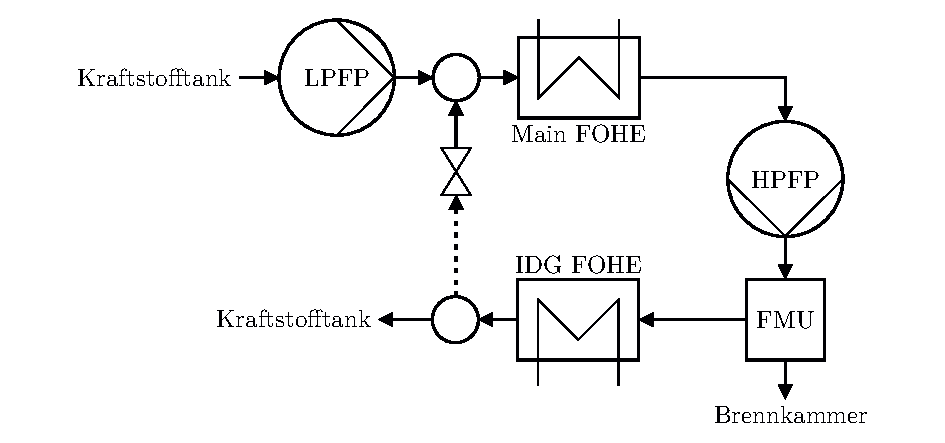
\includegraphics[width=1\linewidth]{4_Abbildungen/2_Hauptteil/Kraftstoffsystem Abbildungen/Referenz.pdf}
  \caption{Kerosin-Kraftstoffsystem}
  \label{fig:Referenz}
\end{figure}
\FloatBarrier 

In dieser Arbeit werden nur Komponenten, die sich innerhalb der Triebwerksgondel befinden, betrachtet. Die Kraftstofftanks und die darin befindlichen Boosterpumpen werden daher nicht modelliert. In der Modellierung wird stattdessen eine Versorgung der Niederdruckpumpe mit dem benötigten Kraftstoffmassenstrom, bei konstanten Eintrittsbedingungen $T_\mathrm{e}, p_\mathrm{e}$ angenommen. 

Die Niederdruckpumpe pumpt den Kraftstoff auf den Austrittsdruck $p_{\mathrm{LPFP}}$ mit dem isentropen Wirkungsgrad $\eta_{\mathrm{LPFP}}$ und einer Leistung von $P_{LPFP}$. Da die Modellierung vorwärts rechnet, ist es nicht möglich die spezifische Enthalpie $h_\mathrm{R}$ des rezirkulierten Kraftstoffs direkt innerhalb derselben Iteration zu integrieren. Stattdessen wird die in der vorherigen Iteration berechnete spezifische Enthalpie verwendet. Der rezirkulierte Kraftstoffmassenstrom $\dot{m}_\mathrm{R}$ wird so gewählt, dass die Brennkammer-Eintrittstemperatur $T_{\mathrm{BK}}$ eingehalten wird. 

Der gemischte Kraftstoffmassenstrom durchläuft anschließend den Wärmeübertrager für das Hauptölsystem und nimmt dabei die Wärme $\dot{Q}_{\mathrm{FOHE}}$ auf. Über diesen Wärmeübertrager liegt ein Druckverhältnis von $\pi_{\mathrm{FOHE}}$ an. Der erwärmte Kraftstoffmassenstrom wird nun in der Hochdruckpumpe mit dem isentropen Wirkungsgrad $\eta_{\mathrm{HPFP}}$ und einer Leistung $P_{\mathrm{HPFP}}$ gepumpt. Der Austrittsdruck der Hochdruckpumpe $p_{\mathrm{HPFP}}$ wird so gewählt, dass der Brennkammer-Eintrittsdruck $p_{\mathrm{BK}}$ erreicht wird.  Da es sich bei der Hochdruckpumpe um eine Verdrängerpumpe handelt und diese für den maximalen Kraftstoffverbrauch im Startfall dimensioniert wird, ist der geförderte Massenstrom im Reiseflug $\dot{m}_{\mathrm{HPFP}}$ vorgegeben. 

Vor dem Eintritt in die Kraftstoffregeleinheit werden in den Leitungen des Kraftstoffsystems auftretende Druckverluste $\Delta p_{\mathrm{L}}$  berücksichtigt. In der Kraftstoffregeleinheit wird der Kraftstoffmassenstrom für die Versorgung der Brennkammer $\dot{m}_{\mathrm{BK}}$ abgezweigt. In den Injektoren erfährt der Kraftstoff den Druckverlust $\Delta p_{\mathrm{inj}}$. 

Der übrige Kraftstoff durchläuft den Wärmeübertrager für das Ölsystem des Stromgenerators und nimmt dabei die Wärme $\dot{Q}_{\mathrm{IDG}}$ auf. Da der rezirkulierte Kraftstoff anschließend gedrosselt wird, wirken sich die Druckverluste dieses Wärmeübertragers nicht auf die Modellierung aus. Nachdem der letzte Wärmeübertrager durchlaufen wurde, wird die spezifische Enthalpie des rezirkulierten Massenstroms berechnet.

\subsection{Variablen und Parameter}

Die abhängigen Variablen des Kerosin-Kraftstoffsystems sind der Brennkammer-Eintrittsdruck $p_{\mathrm{BK}}$ und die Brennkammer-Eintrittstemperatur $T_{\mathrm{BK}}$. Tabelle \ref{Tab:referenz_params} zeigt die Parameter und unabhängigen Variablen des Kerosin-Kraftstoffsystems.

\begin{table}[ht]
    \centering
	\caption{Parameter und Variablen der Modellierung des  Kerosin-Kraftstoffsystems}
	\begin{tabular} {|l|c|l|c|} \hline%
		\multicolumn{2}{|c}{Parameter} & \multicolumn{2}{|c|}{unabhängige Variablen}\\ \hline\hline%
        LPFP-Eintrittstemperatur & $T_\mathrm{e}$ & HPFP-Austrittsdruck & $p_{\mathrm{HPFP}}$ \\ \hline
        LPFP-Eintrittsdruck & $p_\mathrm{e}$ & HPFP-Leistung & $P_{\mathrm{HPFP}}$ \\ \hline
        FOHE-Wärme & $\dot{Q}_{\mathrm{FOHE}}$ & LPFP-Leistung & $P_{\mathrm{LPFP}}$ \\ \hline
        FOHE-Druckverhältnis & $\pi_{\mathrm{FOHE}}$ & rezirkulierter Massenstrom & $\dot{m}_\mathrm{R}$ \\ \hline
        IDG-FOHE-Wärme  & $\dot{Q}_{\mathrm{IDG}}$ & spezifische Enthalpie von $\dot{m}_\mathrm{R}$ & $h_\mathrm{R}$                 \\ \hline
        LPFP-Austrittsdruck & $p_{\mathrm{LPFP}}$& \multicolumn{2}{c|}{}\\ \hline
        isentroper Wirkungsgrad LPFP & $\eta_{\mathrm{LPFP}}$& \multicolumn{2}{c|}{}\\ \hline
        isentroper Wirkungsgrad HPFP & $\eta_{\mathrm{HPFP}}$& \multicolumn{2}{c|}{}\\ \hline
        HPFP-Massenstrom & $\dot{m}_{\mathrm{HPFP}}$& \multicolumn{2}{c|}{}\\ \hline
        Brennkammermassenstrom & $\dot{m}_\mathrm{BK}$& \multicolumn{2}{c|}{}\\ \hline
        Leitungsdruckverluste & $\Delta p_{\mathrm{L}}$& \multicolumn{2}{c|}{}\\ \hline
        Injektordruckverluste & $\Delta p_{\mathrm{inj}}$& \multicolumn{2}{c|}{}\\ \hline
	\end{tabular}	
    \label{Tab:referenz_params}%
\end{table}
\FloatBarrier 

\section{Wasserstoff-Kraftstoffsystemarchitekturen}

Im Folgenden werden unterschiedliche Architekturen für Wasserstoff-Kraftstoffsysteme ausgearbeitet und beschrieben. Abschließend werden die für die Modellierung der Architekturen notwendigen Parameter erläutert. 

Insgesamt werden drei unterschiedliche Kraftstoffsystemarchitekturen betrachtet. Neben einem Kraftstoffsystem mit Hochdruckpumpe werden zwei Systeme mit Verdichter betrachtet. Die beiden Systeme mit Verdichter unterscheiden sich darin, wie sie den Wasserstoff verdampfen. Bei dem Kraftstoffsystem mit Verdampfer wird der Wasserstoff in einem Wärmeübertrager mit Kraftstoff aus dem Hochdrucksystem verdampft. Bei dem Kraftstoffsystem mit Vormischung wird eine geringe Menge Wasserstoff aus dem Hochdrucksystem vor den Verdichter rezirkuliert, um den Kraftstoff vollständig zu verdampfen.

\subsection{Systemarchitektur mit Hochdruckpumpe}

Im Gegensatz zum Kerosin-Kraftstoffsystem wird beim Wasserstoff-Kraftstoffsystem mit Hochdruckpumpe die Funktion der Pumpe nicht auf eine Hochdruck- und eine Niederdruckpumpe mit Wärmeübertragern dazwischen aufgeteilt. Eine Wärmezufuhr hinter einer möglichen Niederdruckpumpe würde den Wasserstoff schon vor der Hochdruckpumpe verdampfen. Die Lösung besteht darin, den Wasserstoff mit einer einzelnen Kreiselpumpe direkt in das Hochdrucksystem zu pumpen und erst daraufhin Wärme zuzuführen. Die hier diskutierte Kraftstoffsystemarchitektur basiert auf einem von Brewer diskutierten Kraftstoffsystem \cite{Brewer.1991}, jedoch wurden keine Wärmeübertrager mit der Turbinenkühlluft und dem Turbinenabgas vorgesehen. Stattdessen versorgt eine parallele Wasserstoffverbrennung den potenziellen Fehlbetrag zwischen dem Wärmebedarf und der verfügbaren Abwärme. Das Wasserstoff-Kraftstoffsystem mit Hochdruckpumpe ist in  Abbildung \ref{fig:pumpe} dargestellt.

\begin{figure}[ht]
\centering
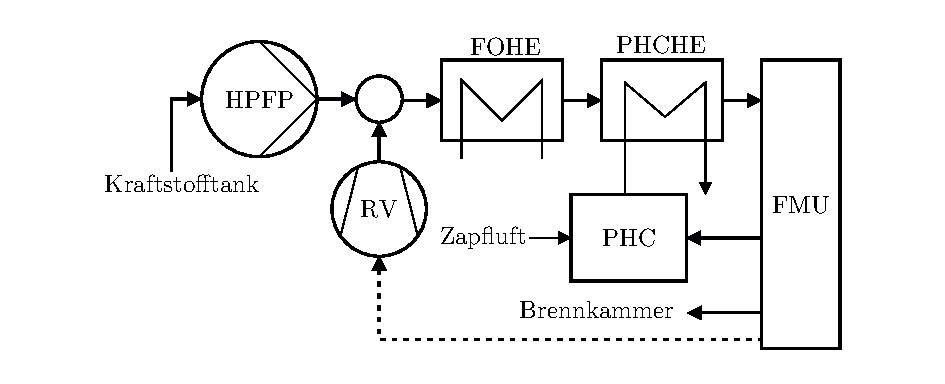
\includegraphics[width=1\linewidth]{4_Abbildungen/2_Hauptteil/Kraftstoffsystem Abbildungen/pump.pdf}
  \caption{Wasserstoff-Kraftstoffsystem mit Pumpe adaptiert aus \cite{Brewer.1991}}
  \label{fig:pumpe}
\end{figure}
\FloatBarrier 

Der Wasserstoff erreicht das Triebwerk im flüssigen Zustand mit dem Eintrittsdruck $p_\mathrm{e}$ und der Eintrittstemperatur $T_\mathrm{e}$ und wird direkt in der Hochdruckpumpe auf den Druck $p_{\mathrm{HPFP}}$ gepumpt, sodass der Brennkammer-Eintrittsdruck $p_{\mathrm{BK}}$ erreicht wird. Die Hochdruckpumpe arbeitet mit dem isentropen Wirkungsgrad $\eta_{\mathrm{HPFP}}$ und benötigt die Leistung $P_{\mathrm{HPFP}}$. 

Um die Druckverluste des rezirkulierten Kraftstoffs im Hochdrucksystem zu kompensieren, schlägt Brewer eine Strahlpumpe mit dem  Hochdruckpumpen-Kraftstoffmassenstrom als Treibmedium vor \cite{Brewer.1991}. Da in dieser Arbeit der rezirkulierte Massenstrom teilweise ein vielfaches des Hochdruckpumpen-Massenstroms beträgt, würde eine Strahlpumpe nicht hinnehmbare Druckverluste verursachen. Stattdessen wird ein Rezirkulationsverdichter (RV) modelliert. Der rezirkulierte Kraftstoffmassenstrom $\dot{m}_\mathrm{R}$ erreicht den Rezirkulationsverdichter mit der Temperatur $T_\mathrm{R}$ und dem Druck $p_\mathrm{R}$ und wird auf den Austrittsdruck der Hochdruckpumpe verdichtet. Der Rezirkulationsverdichter arbeitet mit dem isentropen Wirkungsgrad $\eta_\mathrm{RV}$ und benötigt die Leistung $P_\mathrm{VR}$. 

Der Hodchdruckpumpen-Massenstrom und der rezirkulierte Massenstrom werden anschließend miteinander vermischt. Der warme rezirkulierte Kraftstoff verdampft den flüssigen Kraftstoff aus der Hochdruckpumpe und erwärmt diesen auf die Wärmeübertrager-Eintrittstemperatur $T_\mathrm{W}$, um Vereisungen im Ölsystem zu vermeiden.

Auf den Wärmeübertrager mit dem Klimasystem, folgt der Wärmeübertrager mit dem Ölsystem. Der Einfachheit halber werden die beiden Wärmeübertrager in der Modellierung zusammengefasst. In den beiden Wärmeübertragern wird dem Kraftstoff in Summe die Wärme $\dot{Q}_{\mathrm{FOHE}}$ zugeführt. Über die beiden Wärmeübertrager liegt das Druckverhältnis $\pi_{\mathrm{FOHE}}$ vor. Der durch den Wärmeübertrager mit dem Klimasystem gesparte Fan-Zapfluftbedarf wird in der Modellierung nicht berücksichtigt. Um die angestrebte Brennkammer-Eintrittstemperatur $T_{\mathrm{BK}}$ zu erreichen, wird durch eine parallele Wasserstoffverbrennung (engl.: Parallel Hydrogen Combustion, PHC) in einem weiteren Wärmeübertrager (engl.: PHC Heat Exchanger, PHCHE) die zusätzliche Wärme $\dot{Q}_{\mathrm{PHC}}$ zugeführt. Dieser Wärmeübertrager verursacht das Druckverhältnis $\pi_{\mathrm{PHC}}$. 

Vor dem Eintritt in die Kraftstoffregeleinheit werden in den Leitungen des Kraftstoffsystems auftretende Druckverluste $\Delta p_\mathrm{L}$  berücksichtigt. Die Kraftstoffregeleinheit liefert den Kraftstoffmassenstrom $\dot{m}_{\mathrm{BK}}$ an die Hauptbrennkammer und die Brennkammer der parallelen Wasserstoffverbrennung. Der verbleibender Massenstrom $\dot{m}_\mathrm{R}$ mit der Temperatur $T_\mathrm{R}$ und dem Druck $p_\mathrm{R}$ wird rezirkuliert. Vor dem Eintritt in die Brennkammern erfährt der Wasserstoff die Injektor-Druckverluste $\Delta p_{\mathrm{inj}}$. 

\subsection{Systemarchitektur mit Verdampfer}

Die Architektur mit Verdichter und Verdampfer ist ähnlich wie das Kraftstoffsystem mit Hochdruckpumpe aufgebaut, jedoch wird anstatt der Hochdruckpumpe ein Hochdruckverdichter (engl.: High Pressure Fuel Compressor, HPFC) eingesetzt. Vor dem Eintritt in den Verdichter wird der Wasserstoff in einem Wärmeübertrager mit Wärme aus dem Hochdrucksystem verdampft. Abbildung \ref{fig:verdampfer} zeigt das Kraftstoffsystem mit Verdampfer.

\begin{figure}[ht]
\centering
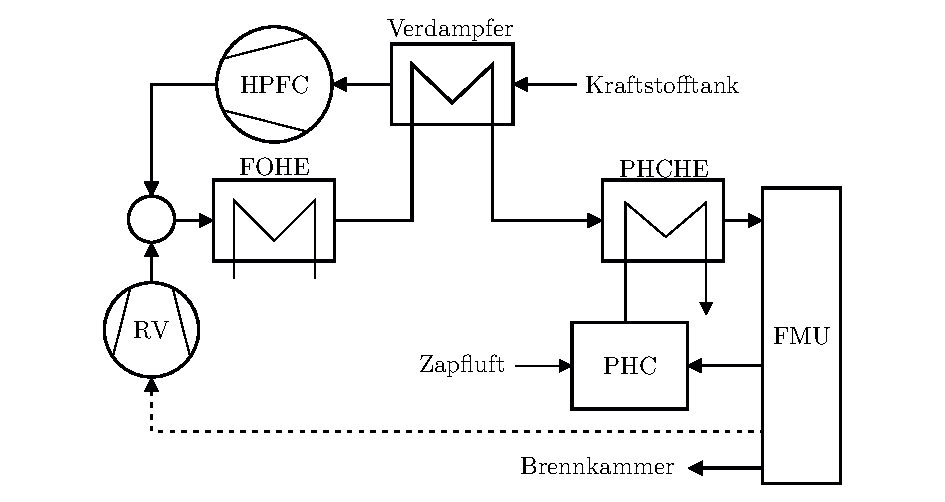
\includegraphics[width=0.85\linewidth]{4_Abbildungen/2_Hauptteil/Kraftstoffsystem Abbildungen/after.pdf}
  \caption{Wasserstoff-Kraftstoffsystem mit Verdichter und Verdampfer}
  \label{fig:verdampfer}
\end{figure}
\FloatBarrier 

Der Wasserstoff wird in dem Triebwerk zunächst in dem Verdampfer unter Zuführung des Wärmestroms $|\dot{Q}_\mathrm{V}|$ aus dem Hochdrucksystem gerade vollständig verdampft. Hierbei liegt über die Niederdruckseite des Wärmeübertragers das Druckverhältnis $\pi_{\mathrm{V,LP}}$ an. Der Hochdruckverdichter fördert den Wasserstoff mit dem Druck $p_{\mathrm{HPFC}}$ in das Hochdrucksystem, sodass der Brennkammer-Eintrittsdruck $p_{\mathrm{BK}}$ erreicht wird. Der Hochdruckverdichter arbeitet mit dem isentropen Wirkungsgrad $\eta_{\mathrm{HPFC}}$ und benötigt die Leistung $P_{\mathrm{HPFC}}$. 

Die Hochdruckseite gleicht dem Kraftstoffsystem mit Hochdruckpumpe mit dem einzigen Unterschied, dass zwischen dem Wärmeübertrager mit dem Ölsystem und dem Wärmeübertrager der parallelen Wasserstoffverbrennung die Hochdruckseite des Verdampfers durchlaufen wird. Hier wird die Wärme $\dot{Q}_\mathrm{V}$ an das Niederdrucksystem abgegeben und es liegt das Druckverhältnis $\pi_{\mathrm{V,HP}}$ an. Der Verdampfer wird auf der Hochdruckseite vor dem Wärmeübertrager mit der parallelen Wasserstoffverbrennung positioniert, um die maximale Wasserstofftemperatur zu mindern. Die geringere Maximaltemperatur ermöglicht eine geringere Abgastemperatur der parallelen Wasserstoffverbrennung und reduziert somit ihren Wasserstoffverbrauch.

\subsection{Systemarchitektur mit Vormischung}

Dieses Kraftstoffsystem hat das Alleinstellungsmerkmal, dass an zwei unterschiedliche Positionen Kraftstoff von der Kraftstoffregeleinheit rezirkuliert wird. Zum einen wie auch bei den anderen Wasserstoff-Kraftstoffsystemen über einen Rezirkulationsverdichter hinter den Hochdruckverdichter. Ein kleiner rezirkulierter Kraftstoffmassenstrom $\dot{m}_\mathrm{V}$ wird jedoch auf den Eintrittsdruck $p_\mathrm{e}$ gedrosselt und vor den Hochdruckverdichter rezirkuliert, um den aus dem Kraftstofftank geförderten Wasserstoff ohne den Einsatz zusätzlicher Wärmeübertrager zu verdampfen. Das Hochdrucksystem des Kraftstoffsystems mit Vormischung unterscheidet sich nicht von dem Kraftstoffsystem mit Hochdruckpumpe (Siehe Abbildung \ref{fig:vormischung}).

\begin{figure}[ht]
\centering
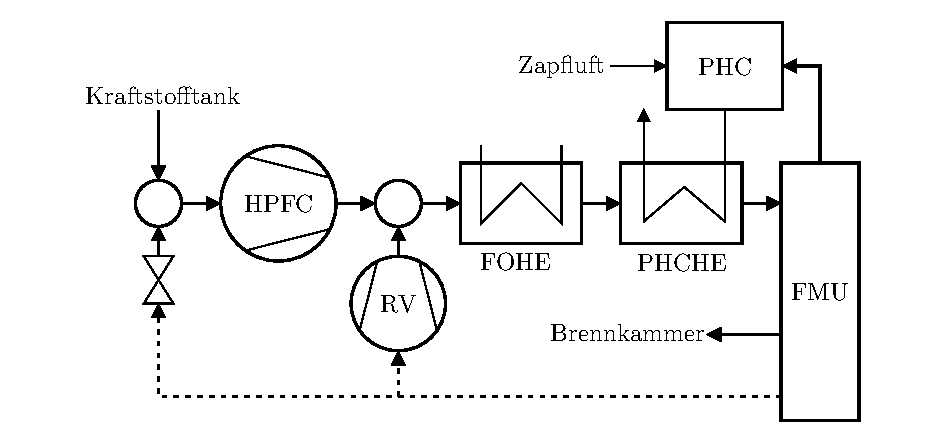
\includegraphics[width=1\linewidth]{4_Abbildungen/2_Hauptteil/Kraftstoffsystem Abbildungen/dual.pdf}
  \caption{Wasserstoff-Kraftstoffsystem mit Verdichter und Vormischung}
  \label{fig:vormischung}
\end{figure}
\FloatBarrier 

\subsection{Variablen und Parameter}

Die abhängigen Variablen der Modellierungen der Wasserstoff-Kraftstoffsysteme sind der Brennkammer-Eintrittsdruck $p_{\mathrm{BK}}$, die Brennkammer-Eintrittstemperatur $T_\mathrm{BK}$ und die Wärmeübertrager-Eintrittstemperatur $T_\mathrm{W}$. Die Parameter und unabhängigen Variablen der Modellierungen sind in Tabelle \ref{Tab:h2_params} zusammengefasst.

\begin{table}[ht]
    \centering
	\caption{Variablen der Modellierungen der Wasserstoff-Kraftstoffsysteme}
	\begin{tabular} {|l|c|l|c|} \hline%
    \multicolumn{4}{|c}{Alle Wasserstoff-Kraftstoffsysteme}\\ \hline
    \multicolumn{2}{|c}{Parameter} & \multicolumn{2}{|c|}{unabhängige Variablen}\\ \hline\hline%
    isentroper Wirkungsgrad RV & $\eta_\mathrm{RV}$ & RV-Leistung & $P_{\mathrm{RV}}$ \\ \hline
    Kraftstoff-Eintrittsdruck & $p_\mathrm{e}$ & rezirkulierter Massenstrom & $\dot{m}_\mathrm{R}$ \\ \hline
    Kraftstoff-Eintrittstemperatur & $T_\mathrm{e}$ & Temperatur des rezirkulierten H$_2$ & $T_\mathrm{R}$ \\ \hline
    PHCHE-Druckverhältnis  & $\pi_{\mathrm{PHC}}$ & Druck des rezirkulierten H$_2$ & $p_\mathrm{R}$\\ \hline
    FOHE-Wärme & $\dot{Q}_{\mathrm{FOHE}}$ & PHCHE-Wärme  & $\dot{Q}_{\mathrm{PHC}}$\\ \hline
    FOHE-Druckverhältnis & $\pi_{\mathrm{FOHE}}$ & \multicolumn{2}{c|}{}\\ \hline
    Brennkammer-Massenstrom & $\dot{m}_\mathrm{BK}$ & \multicolumn{2}{c|}{}\\ \hline
    Leitungs-Druckverluste & $\Delta p_{\mathrm{L}}$ & \multicolumn{2}{c|}{}\\ \hline
    Injektor-Druckverluste & $\Delta p_{\mathrm{inj}}$ & \multicolumn{2}{c|}{}\\ \hline\hline
	\multicolumn{4}{|c|}{Kraftstoffsystem mit Hochdruckpumpe}\\ \hline
    \multicolumn{2}{|c}{Parameter} & \multicolumn{2}{|c|}{unabhängige Variablen}\\ \hline\hline%
    isentroper Wirkungsgrad HPFP & $\eta_{\mathrm{HPFP}}$ & HPFP-Austrittsdruck & $p_{\mathrm{HPFP}}$ \\ \hline
    & & HPFP-Leistung & $P_{\mathrm{HPFP}}$ \\ \hline\hline
    \multicolumn{4}{|c|}{Kraftstoffsystem mit Verdampfer}\\ \hline
    \multicolumn{2}{|c}{Parameter} & \multicolumn{2}{|c|}{unabhängige Variablen}\\ \hline\hline%
    isentroper Wirkungsgrad HPFC & $\eta_{\mathrm{HPFC}}$ & HPFC-Austrittsdruck & $p_{\mathrm{HPFC}}$ \\ \hline
    Druckverhältnis LP-Verdampfer & $\pi_{\mathrm{V,LP}}$ & HPFC-Leistung & $P_{\mathrm{HPFC}}$ \\ \hline
    Druckverhältnis HP-Verdampfer & $\pi_\mathrm{V,HP}$ & Verdampfer-Wärme & $|\dot{Q}_\mathrm{V}|$ \\ \hline\hline
    \multicolumn{4}{|c|}{Kraftstoffsystem mit Vormischung}\\ \hline
    \multicolumn{2}{|c}{Parameter} & \multicolumn{2}{|c|}{unabhängige Variablen}\\ \hline\hline%
    isentroper Wirkungsgrad HPFC & $\eta_{\mathrm{HPFC}}$ & HPFC-Austrittsdruck & $p_{\mathrm{HPFC}}$ \\ \hline
    \multicolumn{2}{|c|}{}& HPFC-Leistung & $P_{\mathrm{HPFC}}$ \\ \hline
    \multicolumn{2}{|c|}{}& Massenstrom Verdampfung & $\dot{m}_\mathrm{V}$ \\ \hline
    \end{tabular}	
    \label{Tab:h2_params}%
\end{table}
\FloatBarrier 


\section{Lösungsalgorithmus}

Im Folgenden wird der Lösungsalgorithmus der in dieser Arbeit entwickelten Methodik exemplarisch am Wasserstoff-Kraftstoffsystem mit Hochdruckpumpe erläutert. Abbildung \ref{fig:algo} stellt den Lösungsalgorithmus des Kraftstoffsystems mit Hochdruckpumpe schematisch als Flussdiagramm dar.

\begin{figure}
\centering
\begin{tikzpicture}[]
	\node (start) [startstop, align = center] {
		Start
	};
	\node (def) [process, below = of start, align = center] {
		Definiere Zielwerte \\ 
		der abhängigen Variablen
	};
	\node (startwerte) [process, below = of def, align=center] 
	{Bestimme Startwerte \\
	der unabhängigen Variablen};
	
	\node (hpfp) [process, below = of startwerte, align = center] {
		Berechne Hochdruckpumpe \\
		Berechne Rezirkulationsverdichter
	};
	
	\node (mix) [process, below = of hpfp, align = center] {
		Berechne Austrittszustand \\ der Kraftstoffmischung
	};
	
	\node (wu) [process, below = of mix, align = center] {
		Berechne Wärmefehlbetrag \\
		Berechne Austrittszustand \\ 
		der Wärmeübertrager 
	};
	
	\node (dp) [process, below = of wu, align = center] {
		Berechne Austrittszustand \\ nach Druckverlusten
	};
	
	\node (phc) [process, right = of dp, align = center] {
		Berechne H$_2$- und Zapfluftbedarf \\
		der parallelen H$_2$-Verbrennung
	};
	
	\node (conv) [decision, above = of phc, align = center] {
		Konvergenz erreicht?
	};
	
	\node (next) [process, right = of hpfp, align = center] {
		Berechne neue Werte \\ der unabhängigen Variablen
	};
	
	\node (end) [startstop, right = of phc] {Ende};
	
	
	\draw [arrow] (start) -- (def);
	\draw [arrow] (def) -- (startwerte);
	\draw [arrow] (startwerte) -- (hpfp);

	\draw [arrow] (hpfp) -- (mix);
	\draw [arrow] (mix) -- (wu);
	\draw [arrow] (wu) -- (dp);
	\draw [arrow] (dp) -- (phc);
	\draw [arrow] (phc) -- (conv);
	\draw [arrow] (conv.north) node[anchor=east] {nein} --  (next);
	\draw [arrow] (next) -- (hpfp);
	%\draw [arrow] (conv.east) -- node[auto] {ja} +(2,0) |- (end);
	\draw [arrow] (conv.east) node[anchor=north] {ja} -|  (end);
	\draw[red, thick] (10.9,-5.5) rectangle (-3.5,-14.2);
	\node[text width=4cm, text=red] at (3.7, -5.2) {Iterationsschleife};
\end{tikzpicture}
\vspace*{0mm}
\caption{Lösungsalgorithmus des Kraftstoffsystems mit Hochdruckpumpe}
\label{fig:algo}
\end{figure}
\FloatBarrier 

Das Verfahren beginnt mit der Definition der abhängigen Variablen $p_\mathrm{BK}$, $T_\mathrm{BK}$ und $T_\mathrm{W}$. Zunächst werden die Startwerte der unabhängigen Variablen $\dot{m}_\mathrm{R}, h_\mathrm{R}, p_\mathrm{HPFP},$ als Funktion der abhängigen Variablen bestimmt. 


